\chapter{Uso de GitHub, Git y JUnit para modificar la librería Materia}\label{chap:github}

Para mayor información sobre la participación en proyectos de GitHub, se recomienda la lectura de las guias:

\begin{itemize}\itemsep0ex
	\item Hola Mundo en GitHub, \url{https://guides.github.com/activities/hello-world/}
	\item Copias personales `Forking', \url{https://guides.github.com/activities/forking/}
	\item Seguimiento de errores y mejoras, \url{https://guides.github.com/features/issues/}
	\item Contribuyendo a proyectos Open-Source, \url{https://guides.github.com/activities/contributing-to-open-source/}
\end{itemize}

Para mayor información sobre Git se recomienda leer la documentación de la página oficial:
\begin{itemize}\itemsep0ex
	\item \url{http://git-scm.com/}
\end{itemize}

Para mayor infomación sobre JUnit se recomienda visitar la página:
\begin{itemize}\itemsep0ex
	\item \url{http://junit.org/}
\end{itemize}

	A continuación se listan brevemente los pasos necesarios para obtener y contribuir a la bliblioteca de clases Materia, es necesario tener una cuenta en GitHub y tener instalados \href{http://git-scm.com/}{Git} y \href{http://maven.apache.org/download.cgi}{Maven} en la computadora.

	\begin{enumerate}\itemsep0ex
		\item Encuentra algo en qué trabajar. Ya sea que encuentres un error en la biblioteca, quieras realizar una mejora o crear una nueva función primero debes estar seguro de lo que quieres hacer. 

		\item Archiva el asunto. Para evitar que dos personas trabajen en el mismo error, o intenten crear funciones semejantes es necesario llevar un registro de lo que se esta realizando en la biblioteca, para ello existe la sección `issues' en la página de GitHub de la biblioteca Materia \url{https://github.com/HugoRedon/Materia}. Ver la figura \ref{fig:issuesMateria}. Para mas información sobre como archivar asuntos en GitHub referirse a la guía de ayuda \url{https://guides.github.com/features/issues/}.

		\begin{figure}[!h]
			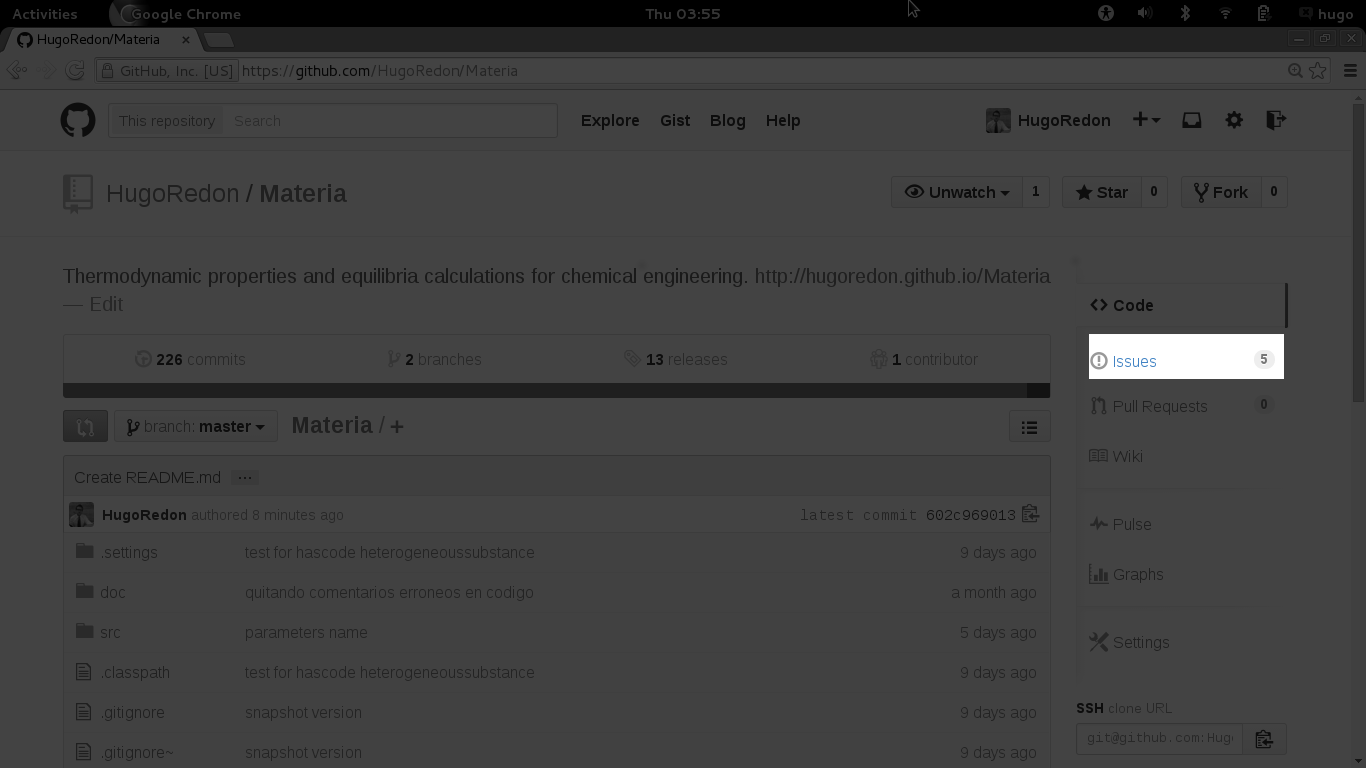
\includegraphics[scale=0.3]{materiaIssues.png}
			\caption{Página de GitHub de la biblioteca Materia, la sección resaltada permite archivar asuntos de error o mejoras en la biblioteca.}
			\label{fig:issuesMateria}
		\end{figure}

		\item Crea una copia personal de la biblioteca en tu cuenta de GitHub `Fork'. Para realizar una copia solo debes dirigirte a la página de GitHub del proyecto \href{https://github.com/HugoRedon/Materia}{Materia} y dar click en el boton `Fork', ver la figura \ref{fig:forkMateria}.

		\begin{figure}[!h]
			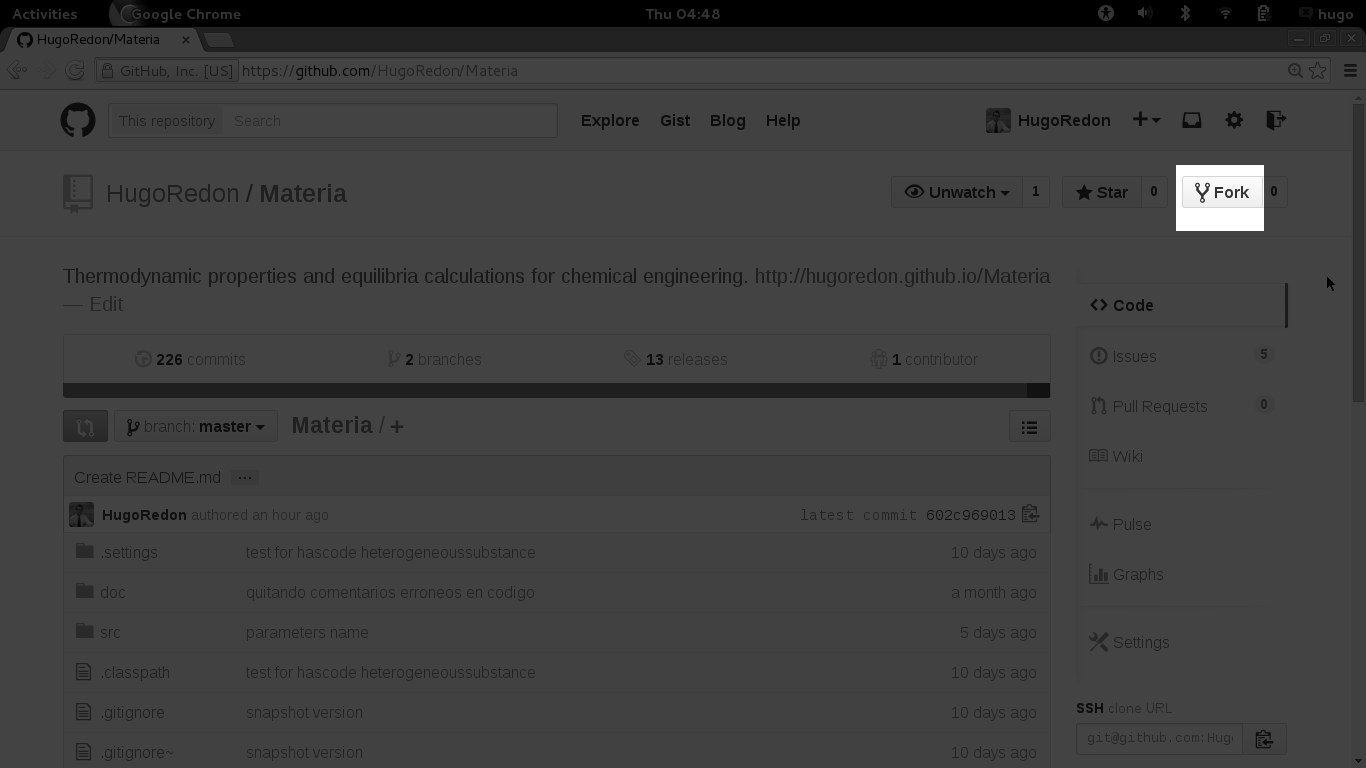
\includegraphics[scale=0.3]{forkMateria.png}
			\caption{Para realizar una copia personal de la biblioteca Materia solo se debe dar click en el boton `Fork'}
			\label{fig:forkMateria}
		\end{figure}

		\item Clona tu copia personal de la biblioteca Materia en tu computadora. 
			\begin{itemize}\itemsep0ex
				\item En github navega a tu copia personal del proyecto Materia
				\item En la barra derecha de la página, da click en el boton 
\includegraphics[scale=0.4]{clonebutton.png} para copiar la url del repositorio.
				\begin{figure}[!h]
					\centering
					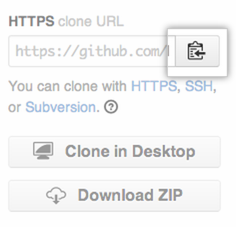
\includegraphics[scale=0.5]{cloneArea.png}.
				\end{figure}
				\item Abre una terminal (para usuarios de Mac y Linux) o linea de comando (usuarios de Windows).
				\item Escribe el comando  `git clone' y después pega la url del paso 2. El resultado debe ser algo semejante al código \ref{lst:cloneCommand}

\begin{lstlisting}[label={lst:cloneCommand},caption={Commando para clonar el repositorio de GitHub},language=bash]
	$ git clone https://github.com/<Nombre de usuario>/Materia
\end{lstlisting}

			\end{itemize}

		\item Crear la rama donde se realizarán los cambios. Para trabajar de forma segura se debe crear una rama donde se desarrollen las nuevas funciones o la corrección a la librería Materia. Esto se logra con el commando \ref{lst:newBranch}. El nombre de la nueva rama debe ser consistente con la tarea a realizar.
		\begin{lstlisting}[label={lst:newBranch},caption={Commando para crear una nueva rama en el repositorio.},language=bash]
			$ git checkout -b <nombre de la nueva rama>
		\end{lstlisting}

		\item Crear las pruebas necesarias que aseguren el funcionamiento del cambio que se desea realizar. El primer paso para resolver un problema es entender el problema. La creación de una prueba ayuda en el proceso de entendimiento del problema. Para ejecutar las pruebas se utiliza el commando de Maven que se muestra en el fragmento de código \ref{lst:mvnTest}. Las pruebas deberán ser creadas en el folder src/test/java dentro del paquete de la clase que se esté probando.

\begin{lstlisting}[caption={Para ejecutar las pruebas del proyecto},label={lst:mvnTest},language=bash]
	$ mvn test
\end{lstlisting}

		Dado que no se ha modificado aún el código, el resultado del comando anterior solo debería encontrar fallas en las pruebas nuevas agregadas.

		\item Escribir las nuevas funciones o las correcciones al código hasta conseguir el éxito en las pruebas. Una vez escritas las pruebas el objetivo del programador es modificar el código hasta que todas las pruebas del código pasen sin errores, es decir que la nueva prueba creada se ejecuta como se esperaba y que ninguna otra prueba ha sido alterada en el proceso.

		\item Agregar los cambios al repositorio local. Si durante el proceso de modificación se agregaron o eliminaron archivos podemos agregar los cambios al repositorio en la computadora mediante los commandos \ref{lst:addCommit}

\begin{lstlisting}[caption={Agregar los cambios al repositorio local.},label={lst:addCommit},language=bash]
	$ git add --all # Agregando los cambios 
	$ git commit -m "<Nota que explique los cambios realizados>" 
		#Archivando los cambios
\end{lstlisting}
		
		Es importante que la nota responda las siguientes preguntas o necesidades:
			\begin{itemize}\itemsep0ex
	 			\item ¿Qué cambios se hicieron al código?
	 			\item ¿Porque se realizaron los cambios al código? ó ¿Qué problema resuelven los cambios agregados? En caso de tener un número de asunto `issue' anotarlo en el comentario, y si este esta resuelto agregar el prefijo fix como se sugiere en la página: \url{https://help.github.com/articles/closing-issues-via-commit-messages}
	 			\item ¿Qué problemas surgieron durante el proceso?
	 			\item ¿Se encontraron otros problemas? si la repuesta es si, entonces listar cuales. De ser necesario crear los asuntos (paso 2) en la página principal de GitHub para ser tratados en el futuro.
		 	\end{itemize}

	 	\item Subir los cambios a la copia personal de GitHub. Hasta este punto solo el repositorio en la computadora contiene los cambios agregados. Para subir los cambios a internet se debe usar el comando \ref{lst:pushMateria}.

	 	\begin{lstlisting}[caption={Comando para agregar los cambios a la copia personal de GitHub},label={lst:pushMateria},language=bash]
	 		$ git push origin master 
	 	\end{lstlisting}

	 	Una vez ejecutado el comando los cambios deberán ser visibles en la página de GitHub, pero estos cambios existen solo en la copia personal.

	 	\item Compartir los cambios al proyecto original.Finalmente si se desea compartir los cambios realizado a la copia personal, es necesario realizar un `pull request', esto se logra dando click en el botón `compare \& pull request' ver la figura \ref{fig:pullRequestMateria}.

	 	\begin{figure}[!h]
	 		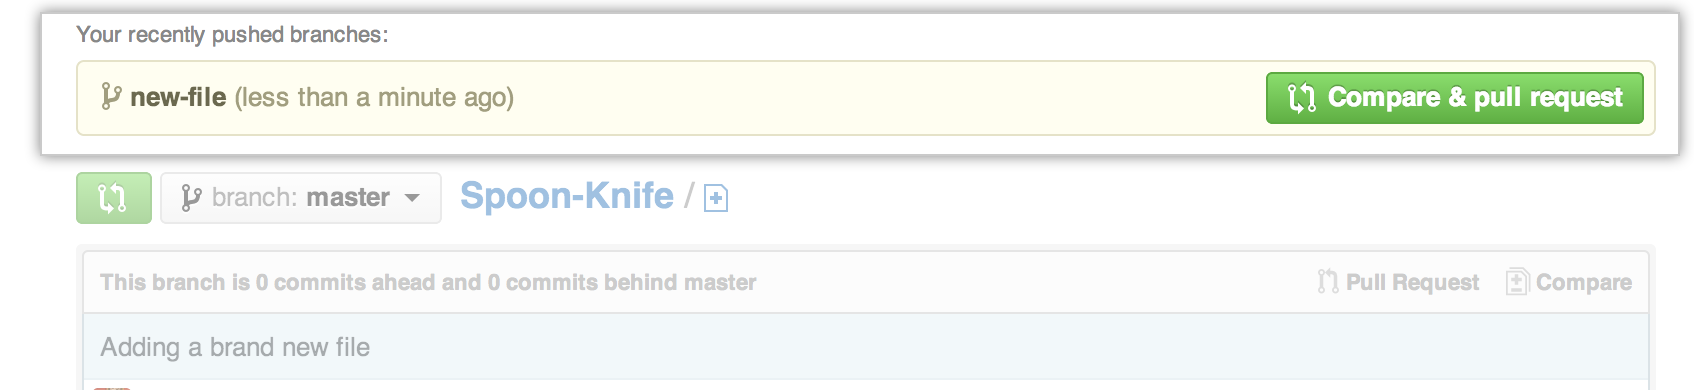
\includegraphics[scale=0.4]{recently_pushed_branch.png}
	 		 \caption{Sección para compartir los cambios al proyecto original.}
	 		 \label{fig:pullRequestMateria}
	 	\end{figure}

	 	Al dar click en el botón serás enviado a una página de discusión donde se debe escribir un título y una descripción sobre la petición para agregar los cambios. Finalmente si los cambios son aceptados habrás concluido tu participación al proyecto Materia y tu perfil de GitHub se habrá agregado a la lista de contribuidores del proyecto Materia.

	\end{enumerate}


